\documentclass{article}
\usepackage{graphicx}
\begin{document}
\begin{center}
	\Large Test 1 Spring
\end{center}
Please read and follow all instructions.
\begin{enumerate}
	\item Sketch the graph of $y=-2x + 6$ including the x and y intercepts.
	\item Solve for $x$:
	$3x + 2 = 23$
	\item Solve for $x$:
	$5x + 1 = 2x - 17$
	\item Find the equation of the line with slope 3 through $(2,5)$
	\textbf{in slope-intercept form}.
	\item Given two points $(1,3)$ and $(4, 12)$:
	\begin{enumerate}
		\item Find the slope of the line connecting them.
		\item Sketch the line.
		\item What is the y-intercept?
	\end{enumerate}
	\item Given $f(x)=x^2+3x+1$, find:
	\begin{enumerate}
		\item $f(2) = ?$
		\item $3 \stackrel{f}{\longmapsto} ?$
		\item $f(-1)=?$
	\end{enumerate}
	\item For the function $f$ given below answer the following questions:
	\newline 
	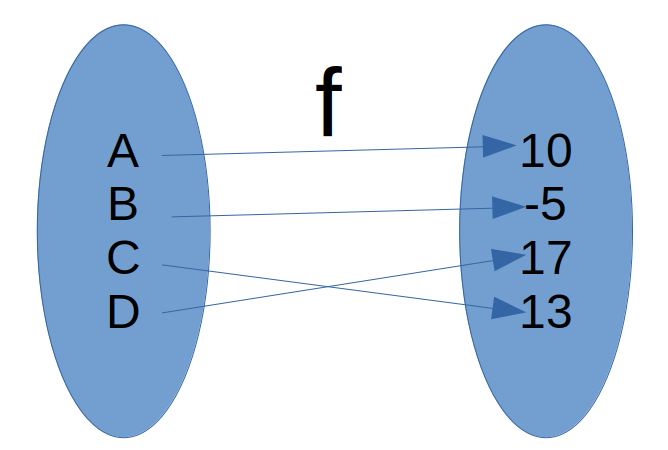
\includegraphics[width=2in]{sptest1_img1.png}
	\begin{enumerate}
		\item $f(A)=?$
		\item $C \stackrel{f}{\longmapsto} ?$
		\item $f(13)=?$
		\item $f(D)=?$
	\end{enumerate}
	\newpage
	\item Find the slope and intercept of the line $4x + 2y = 16$.
	\item Find the slope of a line perpendicular to the line $y=2x - 8$.
	\item For the graph shown below find:
	\begin{enumerate}
		\item The slope
		\item The x intercept
		\item the y intercept
	\end{enumerate}
	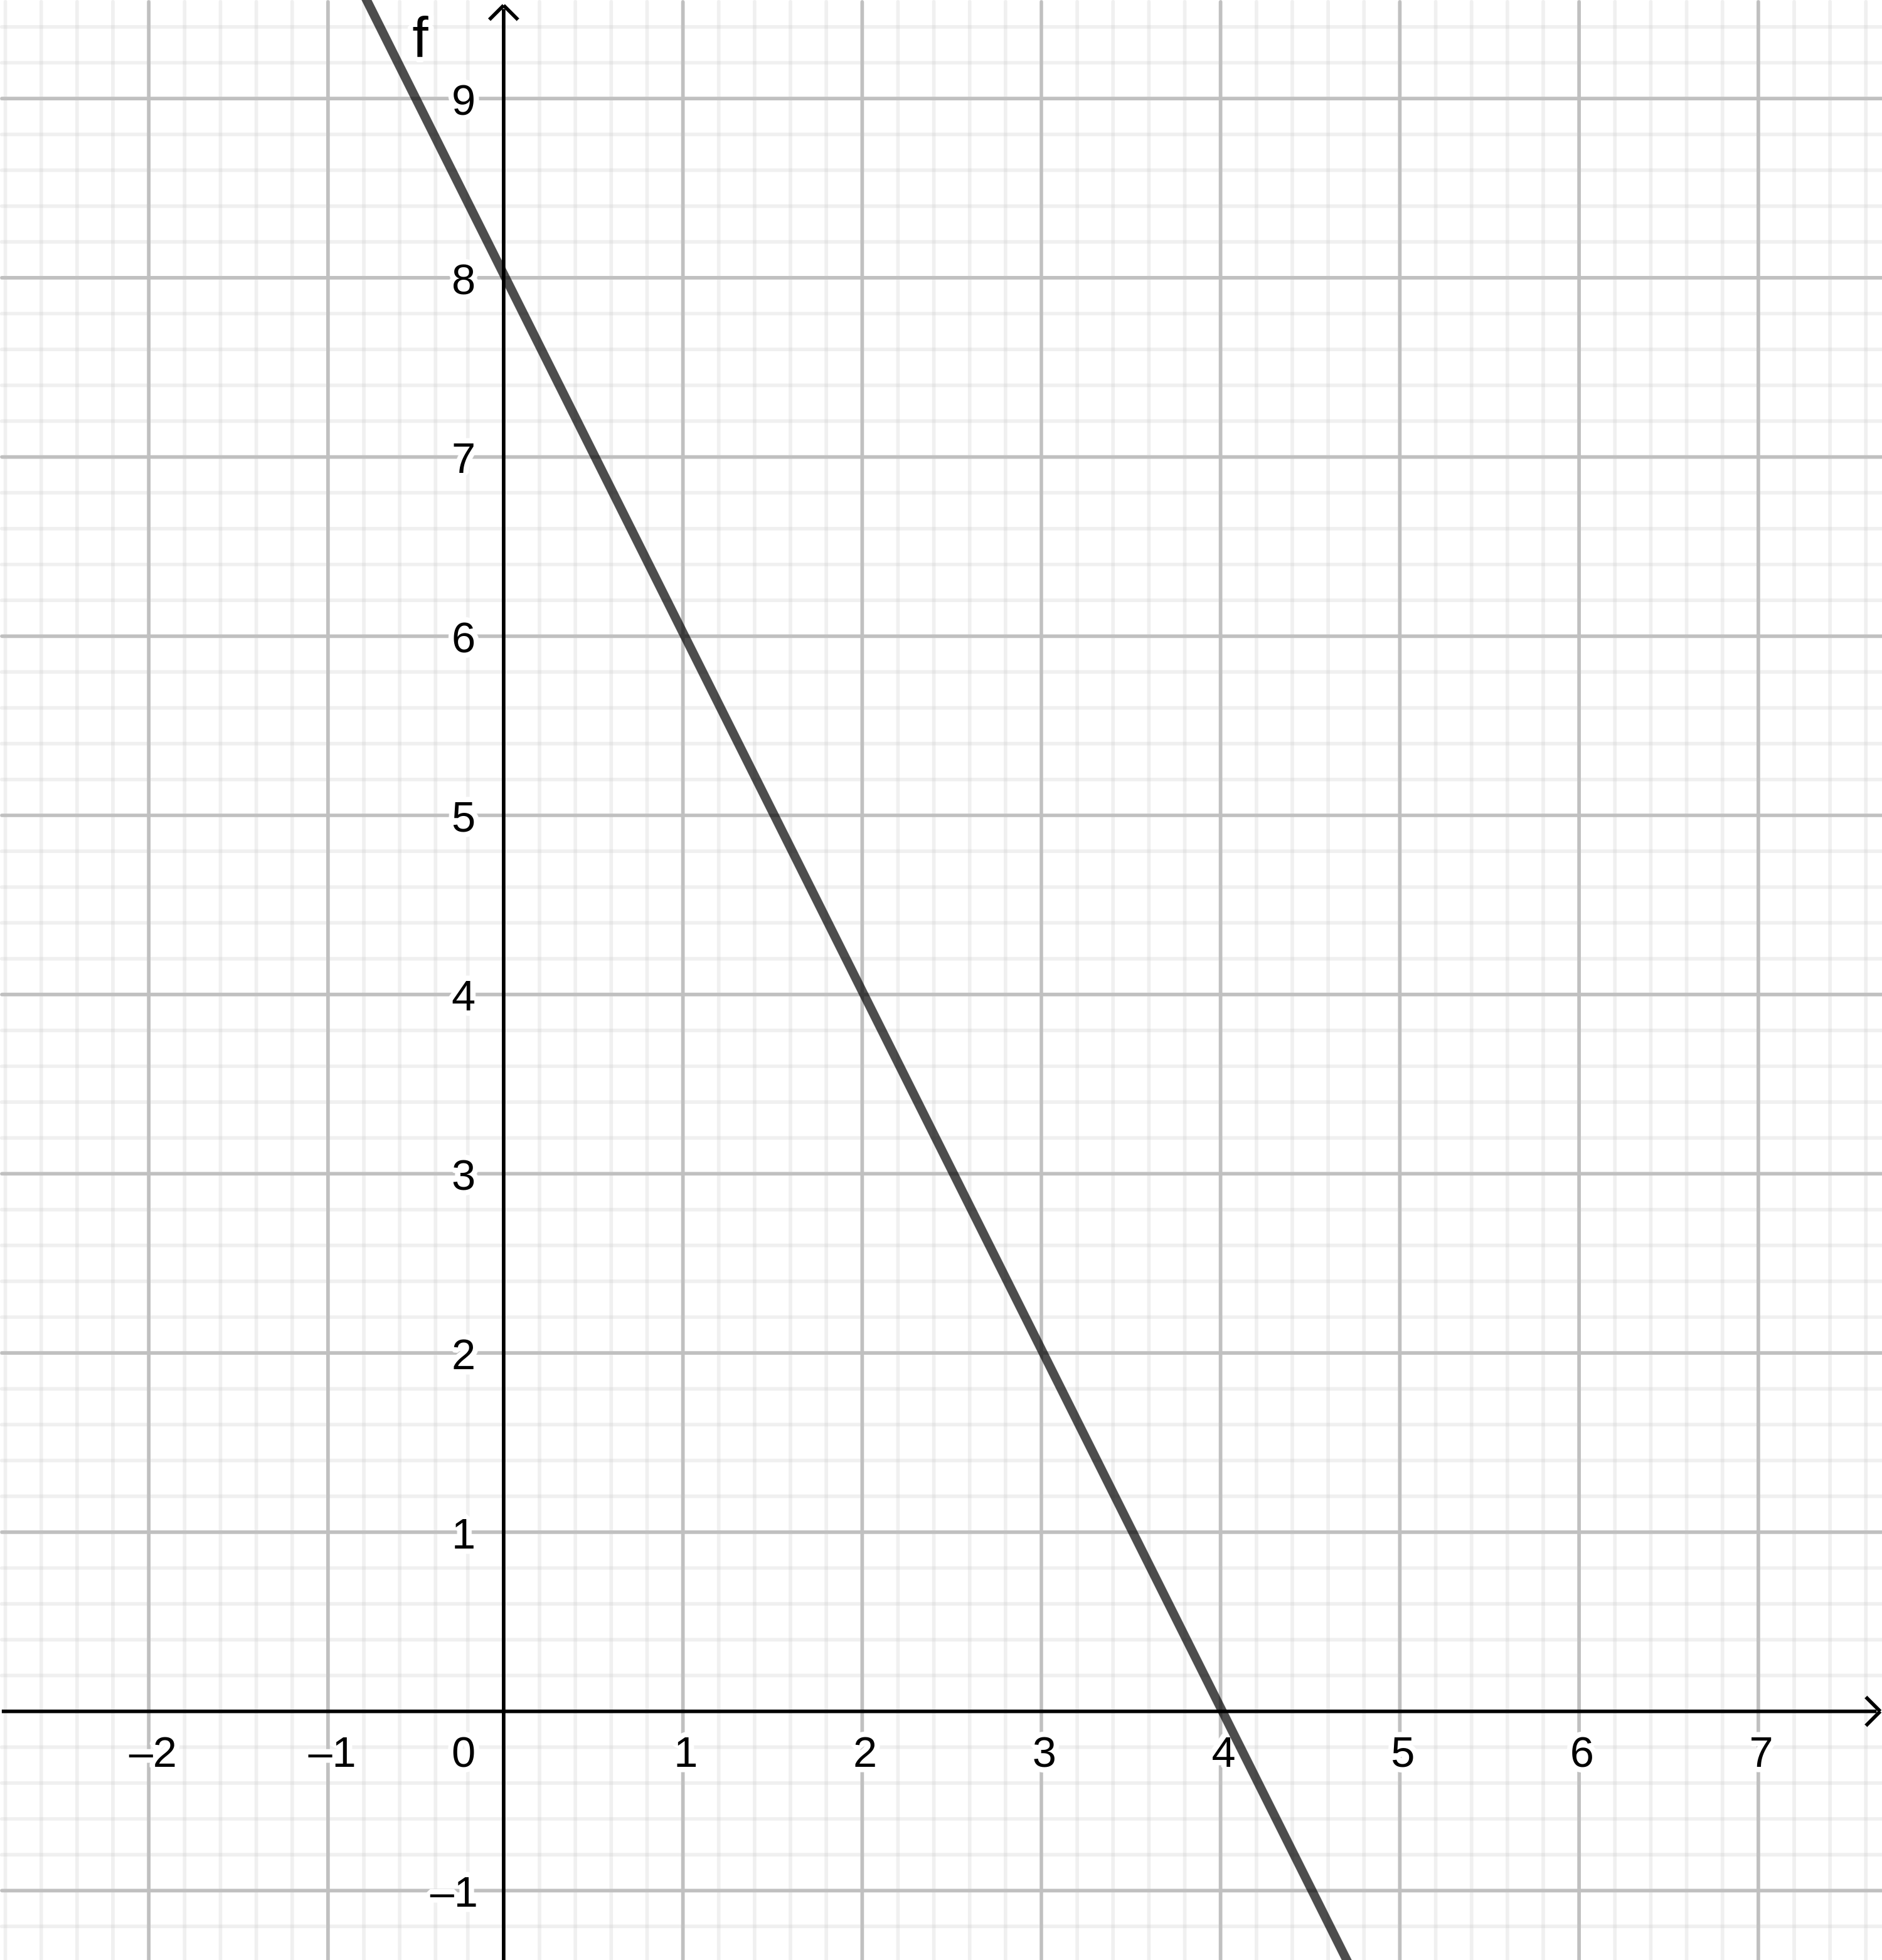
\includegraphics[width=3in]{sptest1_img2.png}
	\item (Extra Credit) Draw a Hitomezashi stitch pattern.
\end{enumerate}
\end{document}